\documentclass[twocolumn]{article}
\usepackage{amsmath}
\usepackage{amssymb}
\usepackage{graphicx}

\begin{document}

\section*{Numbers}

\subsection*{Types of Numbers:}

\begin{itemize}
\item Natural Numbers: $\mathbb{N} = \{1,2,3, \ldots\}$
\item Whole Numbers: $\mathbb{N} \cup \{0\} =\{0,1,2,3, \ldots\}$
\item Integers: $\mathbb{Z} =\{\ldots,-2,-1,0,1,2, \ldots\}$
\item Rational Numbers: $\mathbb{Q} = \left\{\frac{a}{b} \ : \  a, b \in \mathbb{Z} \ , \ b \neq 0 \right\}$. Rational Numbers comprise of fractions (includes all proper and improper fractions and mixed numbers). All terminating decimals (eg, $10.87$) and recurring decimals (eg, $0.3\dot{7}\dot{1} = 0.3717171\ldots$) are rational numbers because these can all be expressed as fractions. All integers are rational numbers.
\item Irrational Numbers: numbers that cannot be expressed in the form $\frac{a}{b}$, where $a$ and $b$ are integers and $b \neq 0$. Eg. $\pi$, $\sqrt{2}$, $\sqrt{5}$, $-4\sqrt{7}$, $e$, $2.75e$, etc. Irrational numbers are non-recurring decimals. Any non-zero rational number multiplied to an irrational number results in an irrational number. For example, $-\frac{3}{4}\pi$ is irrational.
\item Perfect Squares: $\{1,4,9,16,25, \ldots\}$
\item Perfect Cubes: $\{1,8,27,64, \ldots\}$
\item Prime Numbers: Positive integers at least 2 whose only positive divisors are 1 and itself. $\{2,3,5,7,11,13,17,19,23, \ldots\}$
\end{itemize}

\subsection*{Equality and Inequality Symbols}

\begin{tabular}{|c|l|l|}
	\hline Symbol & \multicolumn{1}{|c|}{ Meaning } & \multicolumn{1}{|c|}{ Example } \\
	\hline$=$ & is equal to & $0.1=\frac{1}{10}$ \\
	\hline$\neq$ & is not equal to & $0.11 \neq \frac{1}{10}$ \\
	\hline$>$ & is greater than & $0.1>0.01$ \\
	\hline$\geqslant$ & is greater than or equal to & $a \geqslant 5$ \\
	\hline$<$ & is less than & $0.05<5$ \\
	\hline$\leqslant$ & is less than or equal to & $b \leqslant 5$ \\
	\hline
\end{tabular}

\subsection*{Prime Factorization, HCF, LCM} 

\begin{itemize}
\item Example of prime factorization:

\begin{tabular}{r|c}
	2 & 4356 \\
	\cline { 2 - 2 } 2 & 2178 \\
	\cline { 2 - 2 } 3 & 1089 \\
	\cline { 2 - 2 } 3 & 363 \\
	\cline { 2 - 2 } 11 & 121 \\
	\cline { 2 - 2 } & 11 \\
	\hline 
\end{tabular}

Hence $4356=2^2 \times 3^2 \times 11^2$ (in index notation).

\item Example of HCF and LCM using prime factorization:

$
\begin{aligned}
	& 4800=2^6 \times 3 \times 5^2 \\
	& 5544=2^3 \times 3^2 \times 7 \times 11
\end{aligned}
$

$\mathrm{HCF}=2^3 \times 3$

[take common prime factors and lowest power of each]

$\mathrm{LCM}=2^6 \times 3^2 \times 5^2 \times 7 \times 11$

[take all prime factors and highest power of each]

\item Examples of square roots and cube roots using prime factorization:

$\begin{aligned} 54756 & =2^2 \times 3^4 \times 13^2 \\ \sqrt{54756} & =2 \times 3^2 \times 13 = 234\end{aligned}$

$\begin{aligned} 1728 & =2^6 \times 3^3 \\ \sqrt[3]{1728} & =2^2 \times 3 = 12\end{aligned}$
\end{itemize}

\subsection*{Approximation}

\subsubsection*{Significant Figures}

\noindent
Rules of identifying number of significant digits:

\begin{enumerate} 
\item All non-zero digits are significant.
\item Zeros between non-zero digits are significant. 

Eg. 302 (3 sf)

Eg. 10.2301 (6 sf)

\item In a whole number, zeros after the last nonzero digit may or may not be significant. It depends on the estimation being made.

Eg.

$
\begin{aligned}
	& 7436000=7000000 \ (1 \ \mathrm{sf}) \\
	& 7436000=7400000 \ (2 \ \mathrm{sf}) \\
	& 7436000=7440000 \ (3 \ \mathrm{sf}) \\
	& 7436000=7436000 \ (4 \ \mathrm{sf}) \\
	& 7436000=7436000 \ (5 \ \mathrm{sf}) \\
	& 7436000=7436000 \ (6 \ \mathrm{sf}) \\
\end{aligned}
$

\item In a decimal number, zeros before the $1^{\text{st}}$ non-zero digit are not significant.

Eg. $0.004 \ (1 \ \mathrm{sf})$

Eg. $0.07008 \ (4 \ \mathrm{sf})$

\item In a decimal number, zeros after the last non-zero digit are significant.

Eg. $6.40 \ (3 \ \mathrm{sf})$

Eg. $12.000 \ (5 \ \mathrm{sf})$

Eg. $20300.000 \ (8 \ \mathrm{sf})$

Eg. $0.0700800 \ (6 \ \mathrm{sf})$
\end{enumerate} 

\subsubsection*{Decimal Place Rounding}

\noindent 
Examples:

\noindent
$
\begin{aligned}
	& 0.7374=0.74 \ (2 \ \mathrm{dp}) \\
	& 58.301=58.30 \ (2 \ \mathrm{dp}) \\
	& 207.6296=207.630 \ (3 \ \mathrm{dp}) \\
	& 207.6296=207.63 \ (2 \ \mathrm{dp}) \\
    & 207.977=208.0 \ (1 \ \mathrm{dp}) \\
    & 207.977=207.98 \ (2 \ \mathrm{dp}) \\
    & 18.997=19.00 \ (2 \ \mathrm{dp})
\end{aligned}
$

\subsection*{Standard Form}

\noindent
$\pm A \times 10^n$, where $1 \leq A < 10$ and $n$ is an integer.

\bigskip 

\noindent
Examples:

\noindent
$
\begin{aligned}
	& 1350000=1.35 \times 10^6 \\
	& 0.000375=3.75 \times 10^{-4}
\end{aligned}
$

\subsection*{Common Prefixes}

\begin{tabular}{|l|l|l|l|}
	\hline $10^{12}$ & trillion & tera & $\mathrm{T}$ \\
	\hline $10^9$ & billion & giga & $\mathrm{G}$ \\
	\hline $10^6$ & million & mega & $\mathrm{M}$ \\
	\hline $10^3$ & thousand & kilo & $\mathrm{k}$ \\
	\hline $10^{-3}$ & thousandth & milli & $\mathrm{m}$ \\
	\hline $10^{-6}$ & millionth & micro & $\mu$ \\
	\hline $10^{-9}$ & billionth & nano & $\mathrm{n}$ \\
	\hline $10^{-12}$ & trillionth & pico & $\mathrm{p}$ \\
	\hline
\end{tabular}

\subsection*{Indices}

\noindent 
Rules of Indices:

\bigskip 

\noindent 
Assume that $a,b,m,n$ are non-zero.

\noindent 
$\begin{gathered} a^0=1 \\ a^m \times a^n=a^{m+n} \\ a^m \div a^n=a^{m-n} \\ (a b)^n=a^n b^n \\ \left(\frac{a}{b}\right)^n=\frac{a^n}{b^n} \\ \left(a^n\right)^m=a^{n m} \\ a^{-n}=\frac{1}{a^n} \\ \left(\frac{a}{b}\right)^{-n}=\left(\frac{b}{a}\right)^n=\frac{b^n}{a^n} \\  a^{\frac{1}{n}}=\sqrt[n]{a} \\ a^{\frac{m}{n}}=\sqrt[n]{a^m}=(\sqrt[n]{a})^m\end{gathered}$

\noindent
Caution:

\noindent
1. For indices (powers) that are not integers, the above rules of indices hold only for $a,b > 0$.

\noindent
2. Likewise, if some of the indices are negative or there is division by either $a$ or $b$, then the above rules hold only for $a,b > 0$.

\noindent
3. $\sqrt{(-8)^2} = \sqrt{64} = 8$, NOT $-8$.

\noindent
4. $\sqrt[3]{-27} = -3$.

\bigskip 

\noindent 
Equalities of Indices:

\noindent 
1. If $a^m=a^{\prime \prime}$, then $m=n$.

\noindent 
2. If $a^m=b^m$, then $a=b$.

\subsection*{Percentage, Ratio, Rate}

\begin{itemize}  

\item To express a percentage as a fraction or decimal, divide by $100$:

$
x \%=\frac{x}{100}
$

Eg, $23.5 \% = \frac{23.5}{100} = \frac{235}{1000} = \frac{47}{200}$

Eg, $401 \% = \frac{401}{100} = 4.01$

\item To express any number as a percentage, multiply it by $100 \%$.

Eg, $0.165 = 0.165 \times 100 \% = 16.5 \%$.

\item Expressing a quantity $A$ as a percentage of a quantity $B$:

$
\frac{A}{B} \times 100 \%
$

Eg, Express $63.7$ as a percentage of $98$. 

Answer: $\frac{63.7}{98} \times 100\% = 65 \%$

In words, we say that $63.7$ is $65 \%$ of $98$. 

\item Increase or decrease a quantity by a given percentage:

Eg, Increase $45$ by $2.4 \%$:

Answer: $45 \times \left(1+\frac{2.4}{100}\right) = 45 \times 1.024 = 46.08$  

Eg, Decrease $45$ by $90 \%$:

Answer: $45 \times \left(1-\frac{90}{100}\right) = 45 \times 0.1 = 4.5$

\item Percentage Increase and Percentage Decrease:

When a quantity increases, the percentage increase is

$\frac{\text{final value} \ - \ \text{initial value}}{\text{initial value}} \times 100\%$

When a quantity dereases, the percentage decrease is

$\frac{\text{initial (bigger) value} \ - \ \text{final (smaller) value}}{\text{initial value}} \times 100\%$

Percentage increase will always be $> 0$ if the quantity has increased.

Percentage decrease will always be $> 0$ if the quantity has decreased.

Percentage change is

$\frac{\text{final value} \ - \ \text{initial value}}{\text{initial value}} \times 100\%$

regardless of whether the quantity has increased or decreased. Percentage change can be either positive or negative depending on whether the quantity has increased or decreased.

\item When writing ratios such as $a:b$, $a,b$ are positive integers. Always reduce ratios to the simplest form, eg, $10:6$ is to be reduced to $5:3$. The ratio $a:b$ expressed in fraction form is $\frac{a}{b}$.

Eg, If 7 times of $x$ is equal to 5 times of $y$, then $x:y = 5:7$ (note the switching of the order)

\item We can use ratios to increase and decrease quantities.
For example, if we increase a quantity $x$ in the ratio $6: 5$, the new quantity is $\frac{6}{5} x$; if we decrease a quantity $x$ in the ratio $5: 6$, the new quantity is $\frac{5}{6} x$.

\item Various units of measurement:

Mass:

$1 \ \text{kg} = 1000 \ \text{g}$ 

$1 \ \text{g} = 1000 \ \text{mg}$

Length:

$1 \ \text{km} = 1000 \ \text{m}$

$1 \ \text{m} = 100 \ \text{cm}$

$1 \ \text{cm} = 10 \ \text{mm}$

Area:

$1 \ \text{km}^2 = 10^6 \ \text{m}^2$

$1 \ \text{m}^2 = 10000 \ \text{cm}^2$

Volume:

$1 \ \text{\it l} = 1000 \ \text{ml}$ 

$1 \ \text{cm}^3 = 1 \ \text{ml}$ 

$1 \ \text{m}^3 = 10^6 \ \text{cm}^3 = 1000 \ \text{\it l}$ 

Time:

$1 \ \text{hr} = 60 \ \text{min}$ 

$1 \ \text{min} = 60 \ \text{sec}$ 

\item Distance = Speed $\times$ Time

\item Average speed = (Total Distance) $/$ (Total Time Taken)

\item Conversion of units for speed:

$26 \text{km}/\text{h} = 26000 \text{m}/\text{h} = \frac{26000}{3600}  \text{m}/\text{s} = \frac{65}{9} \text{m}/\text{s} $

$35 \text{m}/\text{s} = 0.035 \text{km}/\text{s} = (0.035 \times 3600) \text{km}/\text{h} = 126 \text{km}/\text{h}$

\item Density = Mass $/$ Volume.

Units are usually $\text{g}/\text{cm}^3$ or $\text{kg}/\text{m}^3$.

$1 \text{g}/\text{cm}^3 = 1000 \text{kg}/\text{m}^3$.

Eg, $0.235 \text{g}/\text{cm}^3 = 235 \text{kg}/\text{m}^3$.

\end{itemize}  

\subsection*{Direct and Inverse Proportion}

\noindent 
If $y$ is directly proportional to $x$, then $y=k x$, where $k$ is a constant and $k \neq 0$. The ratios $\frac{x}{y}$ and $\frac{y}{x}$ are constant. Furthermore, the graph on $y$ against $x$ (or of $x$ against $y$) is a straight line through the origin.

\noindent
Graph showing that $y$ is directly proportional to  $x$:

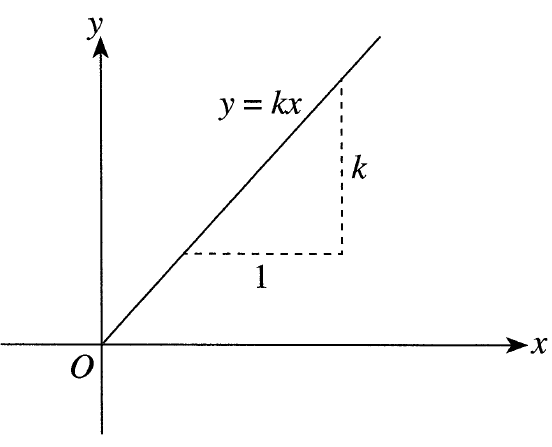
\includegraphics[width=0.3\textwidth]{01.png}

\bigskip 

\noindent 
If $y$ is inversely proportional to $x$, then $y=\frac{k}{x}$, where $k$ is a constant and $k \neq 0$. The product $xy$ is constant. 

\noindent
Graph showing that $y$ is inversely proportional to  $x$:

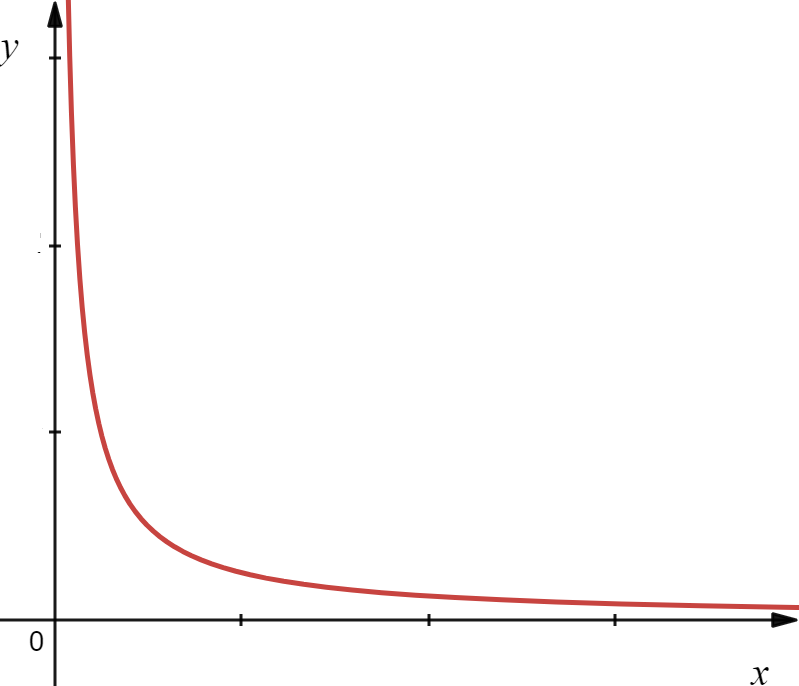
\includegraphics[width=0.3\textwidth]{02.png}

\subsection*{Map Scales}

\begin{itemize}  
	
	\item Linear scale:
	
	$1: n$ means $1$ unit length on map represents $n$ units length on ground.
	
	Eg. $1 : 5000$ means
	
	$1 \mathrm{~cm}$ represents $5000 \mathrm{~cm}$
	
	which implies $1 \mathrm{~cm}$ represents $50 \mathrm{~m}$
	
	which implies $1 \mathrm{~cm}$ represents $0.05 \mathrm{~km}$
	
	\item Representative Fraction (RF):
	
	If the linear scale is $1:n$, the RF is expressed as $\frac{1}{n}$.
	
	Eg, if 3 cm represents 6 m, then RF is $\frac{1}{200}$.
	
	\item Area Scale:
	
	If linear scale is $1:20000$, then it means 
	
	$1 \mathrm{~cm}$ represents $20000 \mathrm{~cm}$
	
	which implies  $1 \mathrm{~cm}$ represents $0.2 \mathrm{~km}$
	
	which implies $1^2 \mathrm{~cm}^2$ represents $(0.2)^2 \mathrm{~km}^2$
	
	which implies $1 \mathrm{~cm}^2$ represents $0.04 \mathrm{~km}^2$

\end{itemize} 

\subsection*{Number Patterns}

\noindent
Common number patterns:

\begin{itemize}  
	
\item Constant difference

Eg, $-5, -2, 1, 4, 7, 10, \ldots$

The $n^{\text{th}}$ term, denoted $T_n$, is given by

$T_n = a + d(n-1)$

where $a$ is the first term and $d$ is the common difference.

For the sequence $-5, -2, 1, 4, 7, 10, \ldots$, 

$T_n = -5 + (n-1)(3) = 3n - 8$.

Alternatively,

$T_n = b + dn$

where $b$ is the term that would have come before the first term (ie, the ``zeroth'' term).

\item Constant multiple (or common ratio)

Eg, $3, 15, 75, 375, \ldots$

$T_n = a \times r^{n-1}$

where $a$ is the first term, $r$ is the common ratio, that is, $r$ is the number that when multiplied a term gives the next term.

For the sequence $3, 15, 75, 375, \ldots$

$T_n = 3 \times 5^{n-1}$.

\item Perfect squares and perfect cubes

$1, 4, 9, 16, 25, \ldots \ : \ T_n = n^2$

$1, 8, 27, 64, 125, \ldots \ : \ T_n = n^3$

$2, 8, 18, 32, 50, \ldots \ : \ T_n = 2n^2$

$3, 10, 29, 66, 127, \ldots \ : \ T_n = n^3+2$
	
\end{itemize}  	

\section*{Algebra}

\subsection*{Simultaneous Linear Equations}

Method 1: Elimination

$
\begin{gathered}
	5 x-2 y=21 \ \ \ \text{---(1)}\\
	2 x-y=8 \ \ \ \text{---(2)}
\end{gathered}
$

$\text{(1)} \times 2: 10 x-4 y=42  \ \ \ \text{---(3)}$

$\text{(2)}\times 5: 10 x-5 y=40  \ \ \ \text{---(4)}$

$\text{(3) - (4)}: \quad y=2$

Sub into (1): $5 x-2(2)=21$

$
\begin{aligned}
	5 x-4 & =21 \\
	5 x & =25 \\
	x & =5
\end{aligned}
$

\bigskip 

\noindent 
Method 2: Substitution

$
\begin{gathered}
	5 x-2 y=21 \ \ \ \text{---(1)} \\
	2 x-y=8 \ \ \ \text{---(2)}
\end{gathered}
$

From (2):

$
y=2 x-8  \ \ \ \text{---(3)}
$

Sub (3) into (1): $5 x-2(2 x-8)=21$

$
\begin{aligned}
	5 x-4 x+16 & =21 \\
	x-16 & =21 \\
	x & =5
\end{aligned}
$

Sub into (2):

$
\begin{array}{r}
	2(5)-y=8 \\
	10-y=8 \\
	y=2
\end{array}
$

\subsection*{Expansion}

\noindent
Eg.

\noindent
$
\begin{aligned}
	& 2 p-3(p+1) \\
	= & 2 p-3 p-3 \\
	= & -p-3
\end{aligned}
$

\noindent
Eg.

\noindent
$
\begin{aligned}
	& 5 x-(x+1)(2 x-3) \\
	= & 5 x-\left(2 x^2-3 x+2 x-3\right) \\
	= & 5 x-2 x^2+3 x-2 x+3 \\
	= & -2 x^2+6 x+3
\end{aligned}
$

\subsection*{Factorization and Identities}

\noindent
Factorization of Quadratic Expressions:

\noindent
$
5 x^2+9 x-2
$

\begin{tabular}{c|c|c|}
	$\times$ & \multicolumn{1}{|c}{$5 x$} & $-1$ \\
	\hline$x$ & $5 x^2$ & $-x$ \\
	\cline { 2 - 3 } $2$ & $10 x$ & $-2$ \\
	\hline 
\end{tabular}

\noindent 
$
\therefore \ \ 5 x^2+9 x-2=(5 x-1)(x+2)
$

\bigskip 

\noindent 
Identities:

\bigskip 

\noindent 
1. $(a+b)^2=a^2+2 a b+b^2$

\noindent 
2. $(a-b)^2=a^2-2 a b+b^2$

\noindent 
3. $(a+b)(a-b)=a^2-b^2$

\bigskip 

\noindent 
Common Factorisation Techniques:

\begin{itemize} 
\item Common Factors

Eg. $6 a^3 b-2 a^2 b=2 a^2 b(3 a-1)$

\item Grouping

Eg.

$
\begin{aligned}
	& 6 p^2-3 p q-10 a p+5 a q \\
	& =3 p(2 p-q)-5 a(2 p-q) \\
	& =(3 p-5 a)(2 p-q)
\end{aligned}
$

\item Using Difference of Two Squares

$
\begin{aligned}
	& \text { Eg. } 9 a^2-1 \\
	& =(3a)^2 - (1)^2 \\
	& =(3 a+1)(3 a-1)
\end{aligned}
$

\noindent 
$
\begin{aligned}
	& \text { Eg. } 16 a^4-81 \\
	& =(4a^2+9)(4a^2-9) \\
	& =(4a^2+9)(2a+3)(2a-3)
\end{aligned}
$

\item Combination of methods:

Eg. $3 x^3-12 x y^2$
$=3 x\left(x^2-4 y^2\right)$ common factor
$=3 x(x+2 y)(x-2 y)$ then diff. of 2 squares

Always try common factor first

Eg.

$
\begin{aligned}
	& 4 - p^2 + 6pq - 9q^2  \\
	& =4 - (p^2 - 6pq + 9q^2) \\
	& =(2)^2 - (p-3q)^2 \\
	& =(2+(p-3q))(2-(p-3q)) \\
	& =(2+p-3q)(2-p+3q)
\end{aligned}
$

\end{itemize} 

\subsection*{Algebraic Fractions}

\noindent 
Eg.

\noindent 
$
\begin{aligned}
	& \frac{x+2}{3}-\frac{x-5}{2} \\
	& =\frac{2(x+2)-3(x-5)}{6} \\
	& =\frac{2 x+4-3 x+15}{6} \\
	& =\frac{19-x}{6}
\end{aligned}
$

\bigskip 

\noindent 
Eg.

\noindent 
$
\begin{aligned}
	& \frac{5}{x+1}-\frac{2}{x-3} \\
	& =\frac{5(x-3)-2(x+1)}{(x+1)(x-3)} \\
	& =\frac{5 x-15-2 x-2}{(x+1)(x-3)} \\
	& =\frac{3 x-17}{(x+2)(x-5)}
\end{aligned}
$

\bigskip 

\noindent 
Eg.

\noindent 
$
\begin{aligned}
	& \frac{5}{3 x}+\frac{2}{x} \\
	& = \frac{5}{3 x}+\frac{6}{3x} \\
	& =\frac{5+6}{3 x} \\
	& =\frac{11}{3 x}
\end{aligned}
$

\bigskip 

\noindent 
Eg. 

\noindent 
$
\begin{aligned}
	& \frac{3}{(x+2)^2}-\frac{4}{x+2} \\
	& =\frac{3}{(x+2)^2}-\frac{4(x+2)}{(x+2)^2} \\	
	& =\frac{3-4(x+2)}{(x+2)^2} \\
	& =\frac{3-4 x-8}{(x+2)^2} \\
	& =\frac{-4 x-5}{(x+2)^2}
\end{aligned}
$

\bigskip 

\noindent 
Eg. 

\noindent 
$
\begin{aligned}
	& \frac{7}{x^2-9}-\frac{1}{x-3} \\
	& =\frac{7}{(x+3)(x-3)}-\frac{1}{x-3} \\
	& =\frac{7}{(x+3)(x-3)}-\frac{x-3}{(x-3)^2} \\	
	& =\frac{7-(x+3)}{(x+3)(x-3)} \\
	& =\frac{7-x-3}{(x+3)(x-3)} \\
	& =\frac{4-x}{(x+3)(x-3)}
\end{aligned}
$

\bigskip 

\noindent 
Eg. 

\noindent 
$
\begin{aligned}
	& \frac{9}{x-5}+\frac{3}{5-x} \\
	& =\frac{9}{x-5}-\frac{3}{x-5} \\
	& =\frac{9-3}{x-5} \\
	& =\frac{6}{x-5}
\end{aligned}
$

\bigskip 

\noindent 
Eg. 

\noindent 
$\begin{aligned} & \frac{2 x}{3 y-8 x}+\frac{11 x}{80 x-30 y} \\ = & \frac{2 x}{3 y-8 x}+\frac{11 x}{-10(3 y-8 x)} \\ = & \frac{2 x}{3 y-8 x}-\frac{11 x}{10(3 y-8 x)} \\ = & \frac{20 x-11 x}{10(3 y-8 x)} \\ = & \frac{9 x}{10(3 y-8 x)}\end{aligned}$

\bigskip 

\noindent 
Eg. 

\noindent 
$\begin{aligned} & \frac{6 p^3}{7 q} \div \frac{2 p}{21 q^2} \\ = & \frac{6 p^3}{7 q} \times \frac{21 q^2}{2 p} \ \ [\text { do cancelling }] \\ = & 9 p^2 q\end{aligned}$

\bigskip 

\noindent 
Eg. 

\noindent 
$\begin{aligned} \frac{4 p q^2+4 p q r}{9 p q r^2+9 p q^2 r} & =\frac{4 p q(q+r)}{9 p q r(r+q)} \\ & =\frac{4}{9 r}\end{aligned}$

\bigskip 

\noindent 
Eg. 

\noindent 
$\begin{aligned} \frac{5 k^2-17 k-12}{5 k^2-10 k-40} & =\frac{(5 k+3)(k-4)}{5\left(k^2-2 k-8\right)} \\ & =\frac{(5 k+3)(k-4)}{5(k-4)(k+2)} \\ & =\frac{5 k+3}{5(k+2)}\end{aligned}$

\bigskip 

\noindent 
Eg. 

\noindent 
$\begin{aligned} & \frac{x y-z^2-x z+y z}{y^2-2 y z+z^2} \div \frac{11}{2 x z+x^2+z^2} \\ & =\frac{x y-x z+y z-z^2}{y^2-2 y z+z^2} \times \frac{2 x z+x^2+z^2}{11} \\ & =\frac{x(y-z)+z(y-z)}{(y-z)^2} \times \frac{(x+z)^2}{11} \\ & =\frac{(x+z)(y-z)}{(y-z)^2} \times \frac{(x+z)^2}{11} \\ & =\frac{(x+z)^3}{11(y-z)}\end{aligned}$

\subsection*{Inequalities}

\noindent 
Inequality sign is reversed when both sides are multiplied or divided by a negative number.

\bigskip 

\noindent 
Eg. $-3x + 4  \geq 12$

$-3x \geq 12-4$

$-3x \geq 8$

$x \leq - \frac{8}{3}$

\bigskip 

\noindent 
Eg. $3(x-1)<4 x+1 \leq 7+2 x$

\bigskip 
\begin{tabular}{c|c} 
$
\begin{aligned}
	& 3(x-1)<4 x+1 \\
	& 3 x-3<4 x+1 \\
	& 3 x-4 x<1+3 \\
	& -x<4 \\
	& x>-4
\end{aligned}
$
& 
$
\begin{aligned}
	& 4 x+1 \leq 7+2 x \\
	& 4 x-2 x \leq 7-1 \\
	& 2 x \leq 6 \\
	& x \leq 3
\end{aligned}
$
\end{tabular} 

\bigskip 

\noindent 
Ans: $-4 < x \leq 3$


\includegraphics[width=0.3\textwidth]{03.png}

\bigskip 

\noindent 
Eg. $5 x+4 \leq 3 x<6-3 x$

\bigskip 
\begin{tabular}{c|c} 
$
\begin{aligned}
	5 x+4 & \leq 3 x \\
	2 x & \leq-4\\
	x & \leq-2
\end{aligned}
$
	& 
$
\begin{aligned}
3 x & <6-3 x \\
6 x & <6 \\
x & <1
\end{aligned}
$
\end{tabular} 

\bigskip 

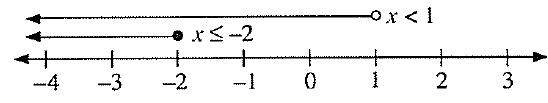
\includegraphics[width=0.45\textwidth]{04.png}

\bigskip 

\noindent 
Ans: $x \leq -2$.


\subsection*{Making Subject of Formula}

\bigskip 

\noindent 
Eg: Make $a$ the subject

\noindent 
$\begin{aligned} y & = m(x-a)+b \\ y-b & =m(x-a) \\ m(x-a) & =y-b \\ x-a & =\frac{y-b}{m} \\ a & =x-\frac{y-b}{m}\end{aligned}$

\bigskip 

\noindent 
Eg: Make $x$ the subject

\noindent 
$\begin{aligned} a x-b y & =3-2 x \\ a x+2 x & =3+b y \\ x(a+2) & =b y+3 \\ x & =\frac{b y+3}{a+2}\end{aligned}$

\bigskip 

\noindent 
Eg: Make $d$ the subject

\noindent 
$\begin{aligned} T & =0.25 \pi d^2 \\ \pi d^2 & =4 T \\ d^2 & =\frac{4 T}{\pi} \\ d & = \pm \sqrt{\frac{4 T}{\pi}}\end{aligned}$

\noindent
Note the $\pm$ when taking square-roots in this type of question.

\bigskip 

\noindent 
Eg: Make $c$ the subject

\noindent 
$\begin{aligned} d & =\frac{8-c}{c+7} \\ d(c+7) & =8-c \\ c d+7 d & =8-c \\ c d+c & =8-7 d \\ c(d+1) & =8-7 d \\ c & =\frac{8-7 d}{d+1}\end{aligned}$

\bigskip 

\noindent 
Eg: Make $q$ the subject

\noindent 
$\begin{aligned} 5 a & =\sqrt{\frac{b^2}{q}-\frac{3 c}{4}} \\ 25 a^2 & =\frac{b^2}{q}-\frac{3 c}{4} \\ \frac{b^2}{q} & =25 a^2+\frac{3 c}{4} \\ \frac{b^2}{q} & =\frac{100 a^2+3 c}{4} \\ \frac{q}{b^2} & =\frac{4}{100 a^2+3 c} \\ q & =\frac{4 b^2}{100 a^2+3 c}\end{aligned}$

\bigskip 

\noindent 
Eg: Make $y$ the subject

\noindent 
$\begin{aligned} \frac{x\left(y z-w^2\right)}{2}-\frac{y}{3} & =6 y \\ 3 x\left(y z-w^2\right)-2 y & =36 y \\ 3 x y z-3 w^2 x-2 y & =36 y \\ 3 x y z-38 y & =3 w^2 x \\ y(3 x z-38) & =3 w^2 x \\ y & =\frac{3 w^2 x}{3 x z-38}\end{aligned}$


\end{document}